\section{Two matroids on a double ray}\label{sec:counterexample}

We now use the local matroid $Q$ from
Theorem~\ref{thm:local-matroid} to construct the required pair.
Recall that $Q=Q^*$ on $E_0=L\mathbin{\dot\cup}R$, where each
of $L,R$ is a labeled copy of the countable set $D$. The ultrafilter
$\mathcal U$ and ordinal rank $\rho$ have the following consequence
for every basis $B$ of $Q$:
\begin{equation}\label{eq:outward-rank}
 B_L\in\mathcal U
 \quad\Longrightarrow\quad
 D\setminus B_R\in\mathcal U
 \quad\text{and}\quad
 \rho(B_L)>\rho(D\setminus B_R).
\end{equation}
The rank is antitone under inclusion of members of $\mathcal U$.
An independent covering will propagate a member of $\mathcal U$
along a ray, strictly decreasing this rank at every step.

\subsection{Direct sums and the common ground set}

For completeness, the direct sums we use satisfy all the infinite-matroid
axioms. Let $(Q_j:j\in J)$ be matroids on pairwise disjoint sets $F_j$,
where $J$ is countable. Declare $I\subseteq\bigcup_{j\in J}F_j$
independent if $I\cap F_j$ is independent in every $Q_j$.
Axioms (I1) and (I2) follow componentwise. The maximal independent
sets are exactly the unions of one basis from each component: a
nonmaximal component permits an extension of the union, and if all
components are maximal no element can be adjoined.

For (I3), if $I$ is not maximal, some $I\cap F_j$ is not maximal
in $Q_j$. Given a global basis $B$, its part $B\cap F_j$ is a
component basis. Apply (I3) there and adjoin the resulting element to
$I$. For (IM), given independent $I\subseteq Y$, choose in each
component a maximal independent extension of $I\cap F_j$ inside
$Y\cap F_j$. Their union is a maximal independent extension of $I$
inside $Y$. These choices are available in ZFC. This proves that the
direct sum is a matroid, and also proves its stated description of
bases. If every component is self-dual on its own labels, then the
complement of each global basis is again a global basis, so the direct
sum is self-dual on the same labels.

Take vertices $v_n$ indexed by $n\in\mathbb Z$. Between $v_n$ and
$v_{n+1}$ put the bundle
\[
 e_n=\{n\}\times D,
 \qquad E=\mathop{\dot\bigcup}_{n\in\mathbb Z}e_n.
\]
Thus every bundle has the fixed label map $(n,d)\mapsto d$ onto $D$.
The ground set $E$ is countably infinite: $D$ is a countably infinite
union of nonempty finite blocks, and $E=\mathbb Z\times D$.
Designate $e_{-1}$, joining $v_{-1}$ and $v_0$, as the central bundle.
At every vertex put a copy $Q_n$ of $Q$ on $e_{n-1}\cup e_n$.
The inward bundle is its $L$-coordinate, and the outward bundle its
$R$-coordinate; explicitly,
\[
\begin{array}{c|cc}
 &L&R\\\hline
 n\le -1&e_n&e_{n-1}\\
 n\ge 0&e_{n-1}&e_n.
\end{array}
\]
Both middle vertices therefore use the central bundle as $L$.
All copies use the same label maps, ultrafilter, and rank.



Define
\[
 M_0=\bigoplus_{n\in 2\mathbb Z}Q_n,
 \qquad
 M_1=\bigoplus_{n\in 2\mathbb Z+1}Q_n.
\]
For either parity, the component supports partition $E$, since each
bundle has exactly one endpoint of that parity. Hence these are
matroids on the same countably infinite set $E$. The preceding
direct-sum verification and $Q=Q^*$ give $M_i=M_i^*$ on the same
labels for $i=0,1$.

The parity placement and inward/outward coordinates are shown in
Figure~\ref{fig:double-ray}.

\begin{figure}[htbp]
\centering
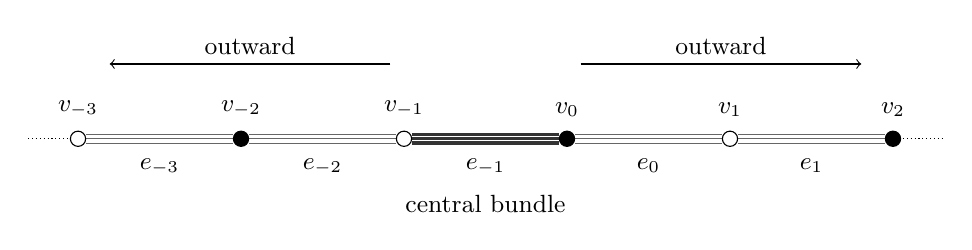
\begin{tikzpicture}[x=1.15cm,y=1cm,font=\small]
  \foreach \a/\b in {-4.5/-2.7,-2.7/-0.9,0.9/2.7,2.7/4.5}{
    \foreach \h in {-0.055,0,0.055}{
      \draw[black!60] (\a+0.09,\h)--(\b-0.09,\h);
    }
  }
  \foreach \h in {-0.055,0,0.055}{
    \draw[very thick,black!80] (-0.81,\h)--(0.81,\h);
  }
  \draw[densely dotted] (-5.05,0)--(-4.61,0);
  \draw[densely dotted] (4.61,0)--(5.05,0);
  \foreach \x/\n in {-4.5/-3,-0.9/-1,2.7/1}{
    \node[circle,draw,fill=white,inner sep=0pt,minimum size=5.5pt]
      at (\x,0) {};
    \node[above] at (\x,0.16) {$v_{\n}$};
  }
  \foreach \x/\n in {-2.7/-2,0.9/0,4.5/2}{
    \node[circle,draw,fill=black,inner sep=0pt,minimum size=5.5pt]
      at (\x,0) {};
    \node[above] at (\x,0.16) {$v_{\n}$};
  }
  \foreach \x/\n in {-3.6/-3,-1.8/-2,0/-1,1.8/0,3.6/1}{
    \node[below] at (\x,-0.13) {$e_{\n}$};
  }
  \draw[->] (-1.05,0.95)--(-4.15,0.95)
    node[midway,above] {outward};
  \draw[->] (1.05,0.95)--(4.15,0.95)
    node[midway,above] {outward};
  \node[below] at (0,-0.59) {central bundle};
\end{tikzpicture}

\caption{Each segment represents a copy of $D$. A copy of $Q$ uses
the two bundles incident with its vertex. Filled vertices contribute
to $M_0$, open vertices to $M_1$. The central bundle is $e_{-1}$;
from either endpoint, the $L$-coordinate points toward the center and
the $R$-coordinate points outward.}
\label{fig:double-ray}
\end{figure}

Every finite subset of $E$ is independent in each $M_i$, because
all its component parts are finite and every finite subset of $Q$ is
independent by Remark~\ref{rem:uniform-local}. But $E$ is dependent
in each $M_i$: its intersection with any component support is the
dependent whole ground set of that copy of $Q$. Thus neither $M_i$
is finitary. Since $M_i=M_i^*$, neither is cofinitary either.

In fact, neither matroid has a nonempty finitary or cofinitary direct
summand. Suppose a nonempty set $F$ supports a finitary summand.
Every subset of $F$ is independent, since all its finite subsets are
independent, so $F$ is the summand's only basis. Thus every basis of
$M_i$ contains $F$. But complements of bases are also bases of $M_i$,
a contradiction. Dualizing the direct-sum basis description gives the
same contradiction for a cofinitary summand.

\subsection{The descending ranks}

Suppose that independent sets $J_i$ of $M_i$ cover $E$.
Replacing $J_1$ by $E\setminus J_0\subseteq J_1$, we obtain an
independent partition $E=J_0\mathbin{\dot\cup}J_1$.
Assign each element of a bundle to the endpoint whose parity agrees
with its part in this partition. At every vertex, the assigned elements
on its two incident bundles form an independent set of its copy of $Q$.

The central bundle is partitioned between $v_{-1}$ and $v_0$.
Exactly one of the two label sets belongs to $\mathcal U$.
Start at that endpoint and move outward forever. Write $x_k\subseteq D$
for the labels received by the $k$th vertex on its inward bundle.
Thus $x_0\in\mathcal U$. If the current vertex receives $z_k$
on its outward bundle, the next vertex receives exactly
\[
 x_{k+1}=D\setminus z_k
\]
there, because the assignment is a partition and the label maps agree.

Assume inductively that $x_k\in\mathcal U$. The independent
assignment at this vertex is contained in a basis $B_k$ of its copy
of $Q$. Put
\[
 u_k=(B_k)_L,
 \qquad y_k=D\setminus(B_k)_R.
\]
We have $x_k\subseteq u_k$, so $u_k\in\mathcal U$.
Equation~\eqref{eq:outward-rank} gives $y_k\in\mathcal U$ and
$\rho(u_k)>\rho(y_k)$. Since $z_k\subseteq(B_k)_R$,
we have $y_k\subseteq x_{k+1}$; hence $x_{k+1}\in\mathcal U$.
Antitonicity now yields
\begin{equation}\label{eq:ordinal-descent}
 \rho(x_k)\ \ge\ \rho(u_k)\ >\ \rho(y_k)\ \ge\
 \rho(x_{k+1}).
\end{equation}
This produces an infinite strictly descending sequence of ordinals,
which is impossible: its set of values has a least element, and the
next value would be smaller.

Thus $M_0,M_1$ have no independent covering of $E$.
By Lemma~\ref{lem:selfdual-reduction}, they have no packing/covering
partition either. Their common ground set is countably infinite and
both matroids are self-dual on the same labels, completing the proof
of Theorem~\ref{thm:main}.
